\section{Dise\~no de Software}

Luego de la eleccion de un microcontrolador, se inicio el proceso de dise\~no. las figuras , , , muestran los diagramas que describen el sistema segun los requerimientos.

\subsection{Descripcion grafica del sistema}
\subsubsection{Diagrama de bloques}
\begin{figure}[h]
  \centering
  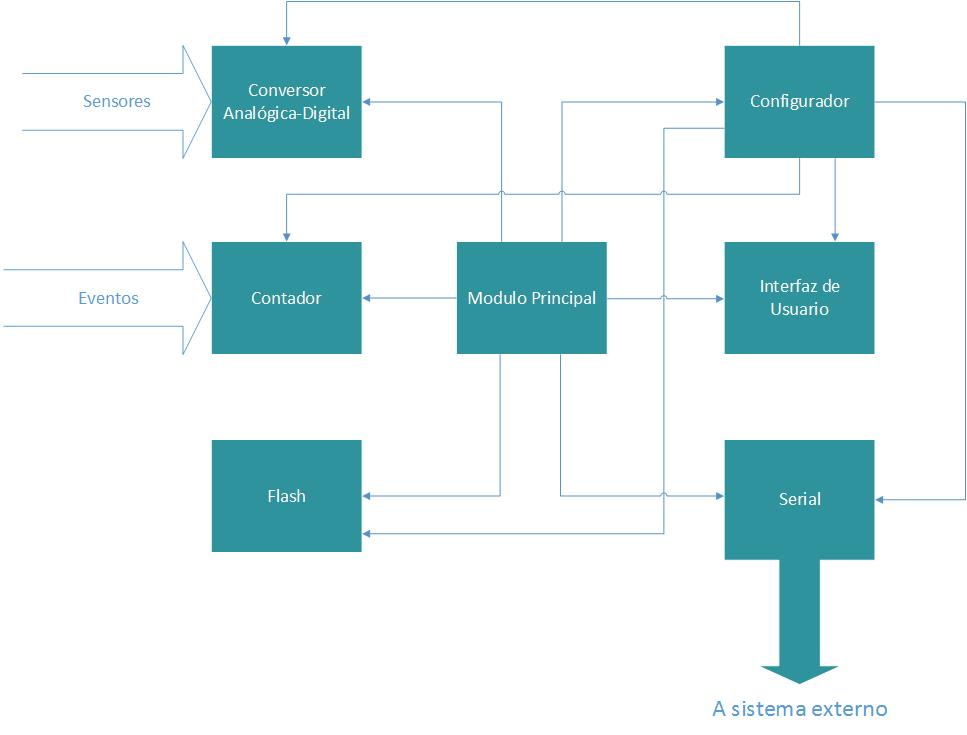
\includegraphics[width=0.80\textwidth, height = 9cm]{Bloques1}
  \caption{Diagrama de Bloques 1}\label{fig:bloques1}
\end{figure}

\paragraph{}
El sistema esta compuesto por 7 bloques o modulos separados, manejados por un modulo principal. En la figura \ref{fig:bloques1} se pueden observar estos bloques y la interaccion que tienen entre si.
\paragraph{}


\begin{itemize}
  \item El \textbf{Bloque Principal} se encarga ejecutar las funciones del resto de los modulos para dar arranque y ejecucion al sistema.
  \item El \textbf{Bloque Conversor Anal\'ogico-Digital} principalmente obtiene los datos de los sensores, los procesa, y los envia al modulo principal. Ademas de esto, configura el funcionamiento del ADC segun los parametros dados por el usuario. El usuario puede elegir la cantidad de pines que va a utilizar como entrada segun la cantidad de sensores que quiera medir, puede elegir un nivel de ganancia de amplificacion de la se\~nal antes de la conversion, y puede tambien elegir el modo de obtencion de los datos (diferencial o single-ended).
  \item El \textbf{Bloque Contador} se encarga de obtener los valores en los contadores de eventos.
  \item El \textbf{Bloque de Interfaz de Usuario} en este modulo se levanta la interfaz con la que interactua el usuario para establecer los parametros configurables del sistema.
  \item El \textbf{Bloque Configurador} interactua directamente con el hardware del microcontrolador. Realiza todas las configuraciones necesarias para poder hacer funcionar cada modulo. Es por esto que en el diagrama de bloques se puede ver que este modulo interactua directamente con todos los demas. Inicializa todos los registros pertinentes, el clock del sistema y setea los puertos de entrada y salida.
  \item El \textbf{Bloque Serial} envia los datos por interfaz serial. Puede ser UART o $I^{2}$C.
  \item El \textbf{Bloque Flash} Maneja la unidad de memoria no volatil del sistema. Se utiliza para guardar y cargar configuraciones hechas por el usuario, de forma que puedan cargarse automaticamente al inicio del sistema sin necesidad de volver a configurarlo cada vez que se inicia.
\end{itemize}

\subsubsection{Diagramas de caso de uso}
En la figura \ref{fig:casouso1} se muestra un diagrama de caso de uso del sistema. Los casos de uso son bastante intuitivos, el usuario debe poder configurar todos los aspectos claves del sistema. Este diagrama muestra a grandes rasgos las acciones posibles que pueden hacerse sobre el sistema desde el punto de vista del usuario.

\begin{figure}[h]
  \centering
  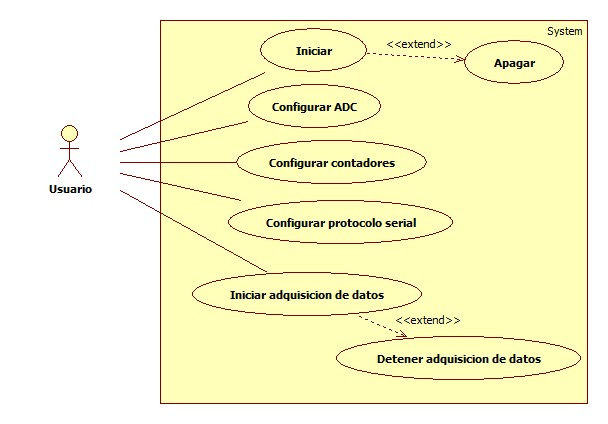
\includegraphics[width=0.80\textwidth, height = 9cm]{CasoUso1}
  \caption{Caso de uso 1}\label{fig:casouso1}
\end{figure}

\subsubsection{Diagramas de secuencia}
Los diagramas de secuencia modelan distintas interacciones entre los componentes de un sistema. En este caso, los dos componentes mas importantes del sistema son el usuario, y el programa principal que recibe las peticiones del usuario a traves de la interfaz grafica, y procesa los pedidos llamando a funciones de otros bloques del sistema. En el primer diagrama (figura \ref{fig:secuencia1}) se modelo una configuracion de un pin especifico para medir una entrada analogica. El programa principal, en este caso, debe llamar a funciones del bloque conversor para configurar el pedido del usuario. Luego, el usuario habilita el comienzo de conversion para que el sistema envie los datos ya digitales por interfaz serial.


\begin{figure}[h]
  \centering
  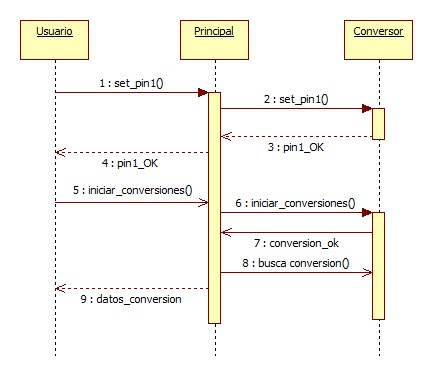
\includegraphics[width=0.50\textwidth, height = 7cm]{Secuencia1}
  \caption{Diagrama de secuencia 1}\label{fig:secuencia1}
\end{figure}

El diagrama en la figura \ref{fig:secuencia2} muestra una configuracion de un contador. En este sistema, los contadores se inician junto con el arranque mismo del sistema y desde ahi mismo comienzan a contar los eventos que ocurran en el pin que tienen asignado. Es por esto que lo unico que hay que hacer es consultar el valor en los registros asociados al contador para obtener la cuenta actual.

El diagrama \ref{fig:secuencia3} muestra una obtencion y un guardado de datos de configuracion en la memoria flash del microcontrolador. Los datos de configuracion son unicamente los pertenecientes al conversor analogico-digital.

\begin{figure}[h]
  \centering
  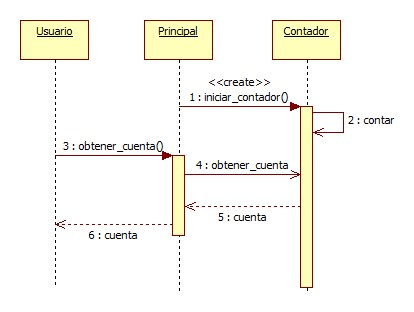
\includegraphics[width=0.50\textwidth, height = 7cm]{Secuencia2}
  \caption{Diagrama de secuencia 2}\label{fig:secuencia2}
\end{figure}


\begin{figure}[H]
  \centering
  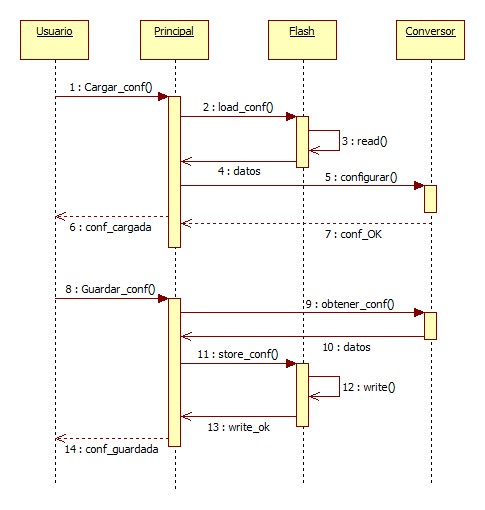
\includegraphics[width=0.60\textwidth, height = 8cm]{Secuencia3}
  \caption{Diagrama de secuencia 3}\label{fig:secuencia3}
\end{figure}

\clearpage